\documentclass{beamer}
\usepackage[autokw=all]{svn-multi}
\setbeamertemplate{navigation symbols}{}
%\usetheme{Goettingen}
\usetheme{Malmoe}
\usefonttheme{default}
%\setbeamersize{text margin left=5pt,text margin right=5pt}

\usepackage{hyperref}
\usepackage{subfigure}
\usepackage{amsmath}
\usepackage{amssymb}
\usepackage{multimedia}
\usepackage{shadow}
%\usepackage{movie15}

\usepackage{tcolorbox}

% Create a ``Wider'' command to reduce margins.  Put
% ``\Wider{\lipsum[2]}'' in a frame...
\newcommand\Wider[2][3em]{%
\makebox[\linewidth][c]{%
  \begin{minipage}{\dimexpr\textwidth+#1\relax}
  \raggedright#2
  \end{minipage}%
  }%
}

\tcbset{ % colback=blue!5,colframe=blue!75!black,
    noparskip,
    colback=blue!5, %background color of the box
    colframe=blue!70, %color of frame and title background
    coltext=black, %color of body text
    coltitle=black, %color of title text 
    fonttitle=\bfseries,
    update/.style={coltitle=red, 
                     colframe=gray!40},
    quote/.style={coltitle=gray!20, 
                     colframe=black,             
                     colback=green!5},
    }


%\usepackage[english]{babel}
%\usepackage{pgf,pgfarrows,pgfnodes,pgfautomata,pgfheaps}
% \usepackage[latin1]{inputenc}

\usepackage{graphicx}
\defbeamertemplate*{footline}{default theme}
{
  \leavevmode%
  \hbox{%
  \begin{beamercolorbox}[wd=.5\paperwidth,ht=2.25ex,dp=1ex,center]{author in head/foot}%
    %\usebeamerfont{author in head/foot}\insertshortauthor~~(\insertshortinstitute)
    \usebeamerfont{author in head/foot}\insertshortauthor
  \end{beamercolorbox}%
  \begin{beamercolorbox}[wd=.4\paperwidth,ht=2.25ex,dp=1ex,center]{title in head/foot}%
    \usebeamerfont{title in head/foot}\insertshorttitle
  \end{beamercolorbox}%
  \begin{beamercolorbox}[wd=.1\paperwidth,ht=2.25ex,dp=1ex,right]{date in head/foot}%
%    \usebeamerfont{page number}\insertframenumber{} / \inserttotalframenumber\hspace*{2ex} 
    \usebeamerfont{page number}\insertpagenumber{} / \insertpresentationendpage{} \hspace*{2ex} 
  \end{beamercolorbox}}%
  \vskip0pt%
}

\title[AlphaGo]{AlphaGo}

\author{Ben Pearre}
%\institute[]{
%  Computer Science\\
%  University of Colorado at Boulder, USA}
\date{\today}
%\date{\today}

\begin{document}

%\begin{frame}
%  \titlepage
%\end{frame}

%\begin{frame}
%  \frametitle{Outline}
%  \tableofcontents
%\end{frame}

\begin{frame}[plain,label=Kasparov]
  \begin{center}
    \includegraphics<+>[width=\textwidth]{knot}
    \includegraphics<+>[width=\textwidth]{knot_closeup}
    \includegraphics<+>[width=\textwidth]{darwin}
    \includegraphics<+>[width=\textwidth]{Go-players}
    \includegraphics<+>[width=\textwidth]{ZhongguoMeishuQuanji}
    \includegraphics<+>[width=\textwidth]{Wenwu_1189}
    \includegraphics<+>[height=\textheight,keepaspectratio]{Go-fight}
    \includegraphics<+>[width=\textwidth]{Sedol-Alphago}
  \end{center}
\end{frame}

%\begin{frame}
%  \outline
%\end{frame}


\section{Go and Machines}

\subsection{Go tutorial}

\begin{frame}
  \frametitle{Go tutorial\dots}
  \begin{center}
    \href{http://playgo.to/index-e.html}{\beamergotobutton{The Way To Go}}
  \end{center}
\end{frame}

\subsection{Machine gameplay with Minimax}

\begin{frame}
  \frametitle{Machine play with Minimax:}
  \begin{center}
    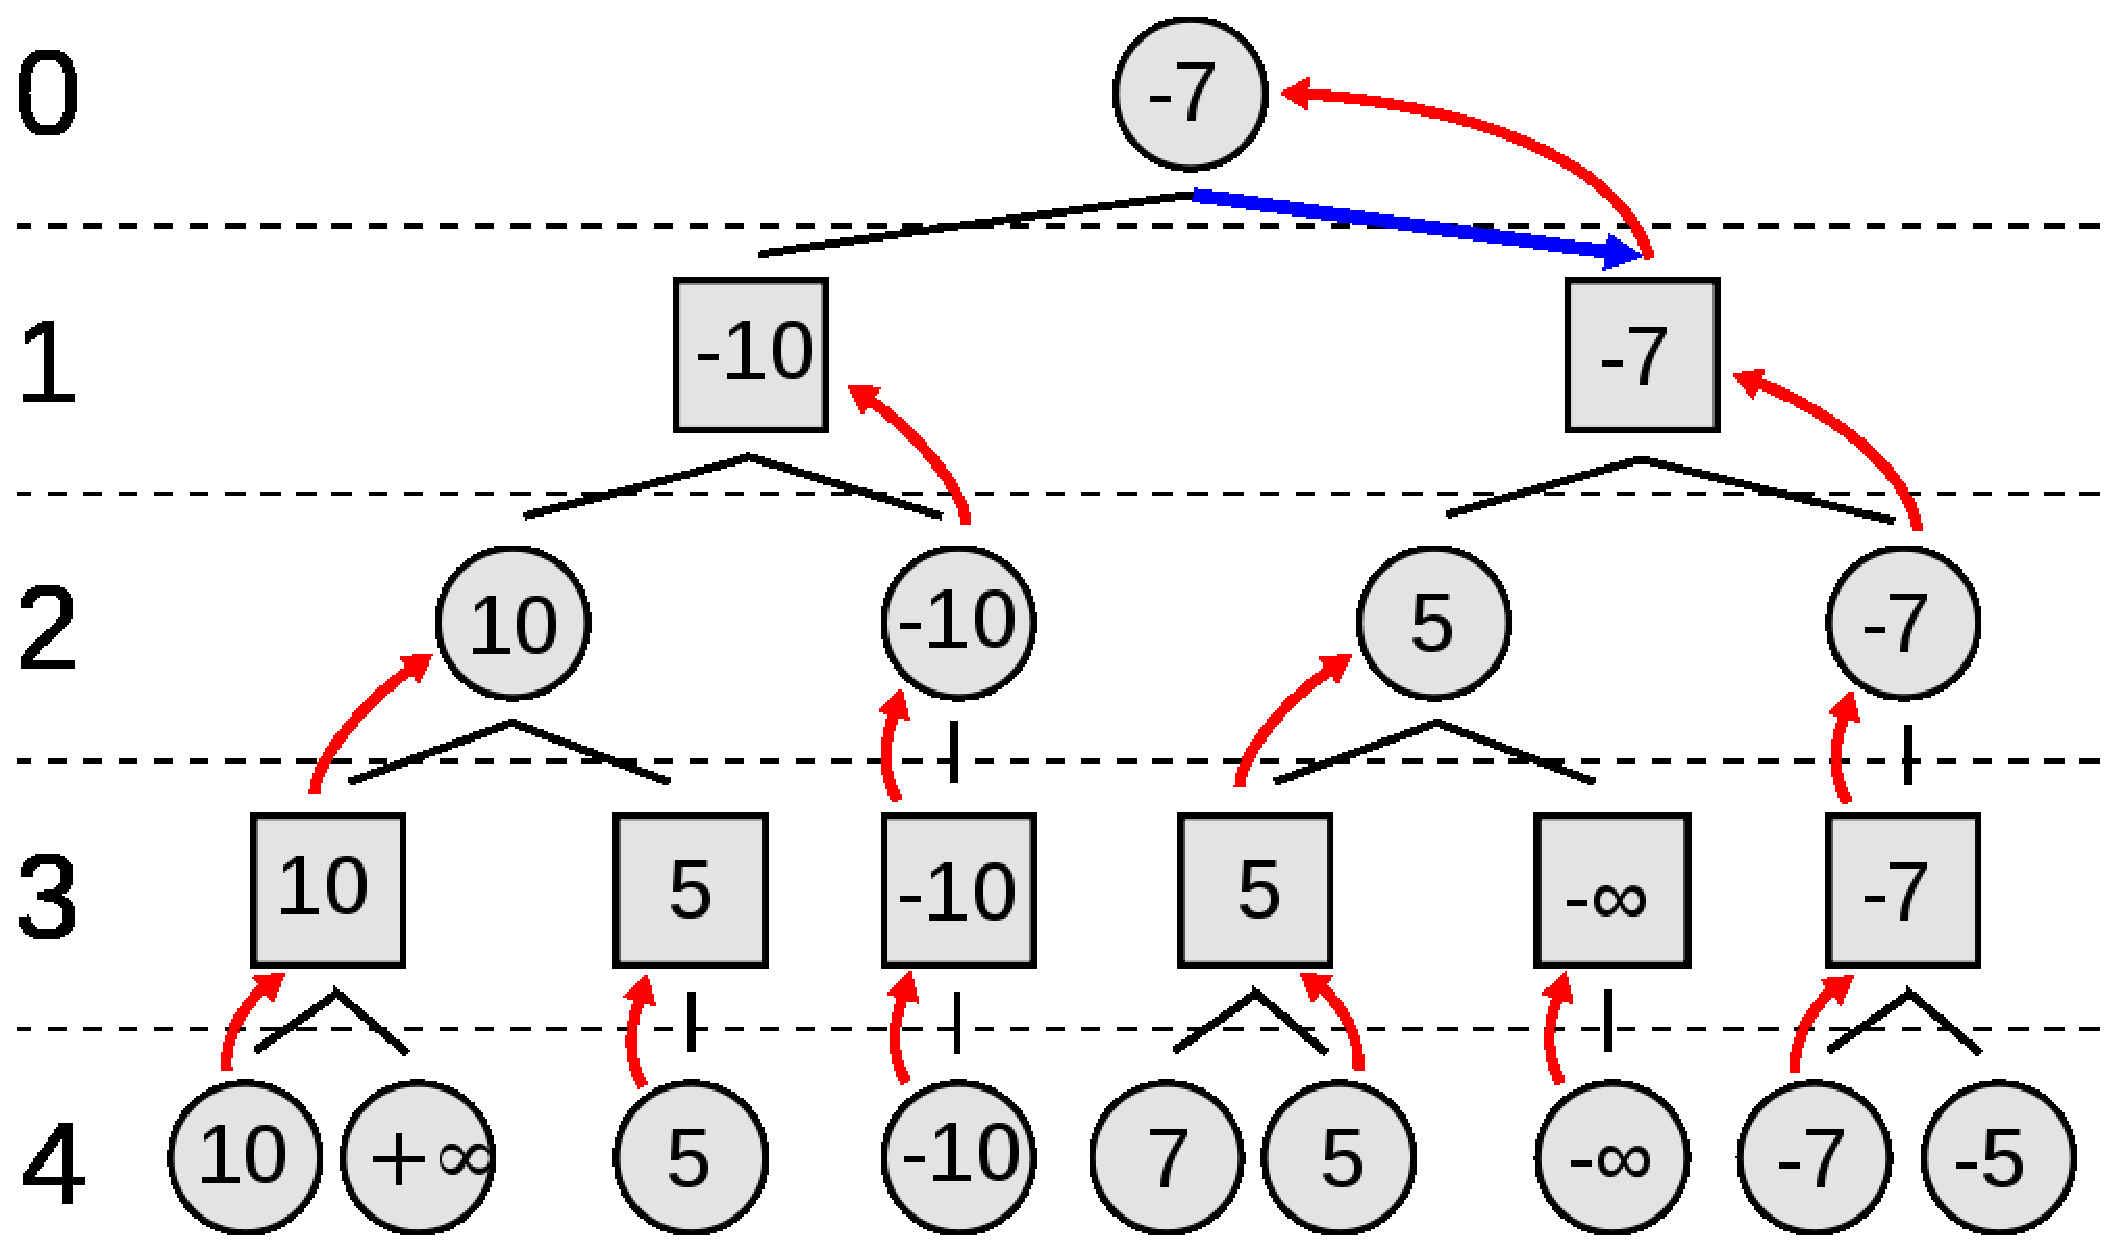
\includegraphics[width=\textwidth]{minimax}
  \end{center}
\end{frame}

\begin{frame}
  \frametitle{How big is the game tree?}
  \begin{description}
  \item[Branching factor:] At each position, $n$ possible moves
  \item[Length:] game lasts $m$ moves
  \end{description}
  \vskip 1 cm
  \begin{tcolorbox}
    \begin{center}
      $n^m$ possible games
    \end{center}
  \end{tcolorbox}
\end{frame}


\begin{frame}
  \frametitle{Size of games}
  \begin{tabular}{l|ccc}
    Game & Branching factor & Length & $\log_{10}\mbox{(\# Games)}$\\ \hline
    Tic-Tac-Toe & 4 & 9 & 5 \\
    Connect Four & 4 & 36 & 21 \\
    Checkers ($8\times 8$) & 2.8 & 70 & 31 \\
    Chess & 35 & 70 & 108 \\
    Backgammon & 250 & 55 & 132 \\
    Carcassonne & 55 & 71 & 195 \\
    Go & 250 & 150 & 360
  \end{tabular}
\end{frame}


\begin{frame}
  \frametitle{Reducing the computational complexity}
  \begin{description}
  \item[Length:]\hfill
    \begin{itemize}
    \item Estimate the value of non-terminal states
    \end{itemize}
  \item[Branching factor:]\hfill
    \begin{itemize}
    \item $\alpha$-$\beta$ Pruning
      \begin{itemize}
      \item $O\left(\sqrt{n^m}\right)$ if moves are sorted
      \end{itemize}
    \item Monte Carlo Tree Search {\em of promising moves}
    \end{itemize}
  \end{description}
\end{frame}



\begin{frame}
  \frametitle{Estimating the value of non-terminal states}
  \begin{description}
  \item[Checkers:]\hfill
    \begin{itemize}
    \item Material
    \item Position of non-kings
    \end{itemize}
  \item[Chess:]\hfill
    \begin{itemize}
    \item Material
    \item Mobility
    \item Control centre of board
    \end{itemize}
  \item[Go:]\hfill
    \begin{itemize}
    \item ``Strength'' / ``Influence''
      \begin{itemize}
      \item Um\dots
      \end{itemize}
    \end{itemize}
  \end{description}
  \begin{tcolorbox}
    \begin{center}
      Intuition!
    \end{center}
  \end{tcolorbox}
\end{frame}


\subsection{Monte Carlo Tree Search}

\begin{frame}<1>[label=mcts]
  \frametitle{Monte Carlo Tree Search \only<2>{II}}
  \includegraphics<1>[width=\textwidth]{MCTS}
  \includegraphics<2>[width=\textwidth]{MCTS-go}
  
  \begin{columns}
    \column{0.75\textwidth}
    \begin{tcolorbox}[title=Selecting a move for roll-out]

      \begin{columns}
        \column{0.7\textwidth}
        Early:
        \begin{itemize}
        \item High prior probability\only<1>{?} \only<2>{from $p_\sigma(s,a)$!}
        \item Low visit count
        \end{itemize}
        
        \column{0.3\textwidth}
        Later:
        \begin{itemize}
        \item Success rate
        \end{itemize}
      \end{columns}
    \end{tcolorbox}

    \column{0.25\textwidth}
    \begin{tcolorbox}[title=Return]
      The most visited move
    \end{tcolorbox}
  \end{columns}
\end{frame}


\begin{frame}
  \frametitle{Ignoring questionable moves}
  Only examine promising moves.
  \vskip 1 cm
  \begin{tcolorbox}[title=Intuition]
    In the beginner's mind there are many possibilities. In the expert's mind there are few. --Shunryu Suzuki
  \end{tcolorbox}
\end{frame}


\subsection{Convolutional neural networks}

\begin{frame}
  \frametitle{Neural Networks}
  \begin{columns}
    \begin{column}{0.5\textwidth}
      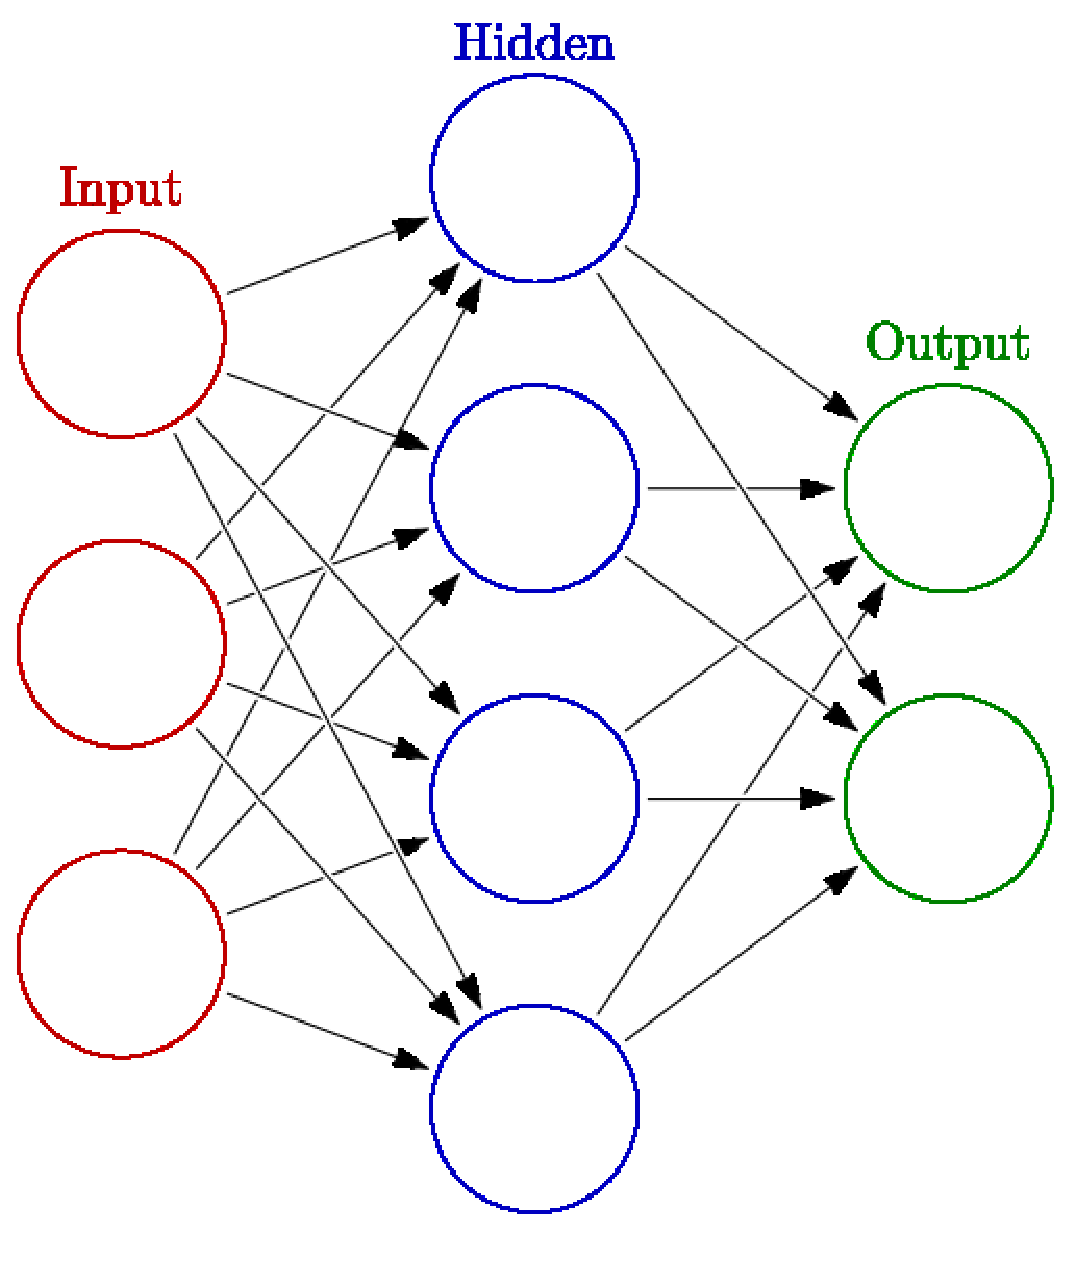
\includegraphics[width=0.8\textwidth]{neural_network}
    \end{column}
    \begin{column}{0.5\textwidth}
      \begin{itemize}
      \item Input pattern $\xi$
      \item Weights $W$
      \item $y = W_1 \tanh (W_0 \xi) $
      \item $W_i$ are trained with backpropagation of errors
      \end{itemize}
    \end{column}
  \end{columns}
\end{frame}

\begin{frame}
  \frametitle{Convolutional Neural Networks}
  Inspired by Hubel \& Wiesel 1968?
  \vskip 1 cm
  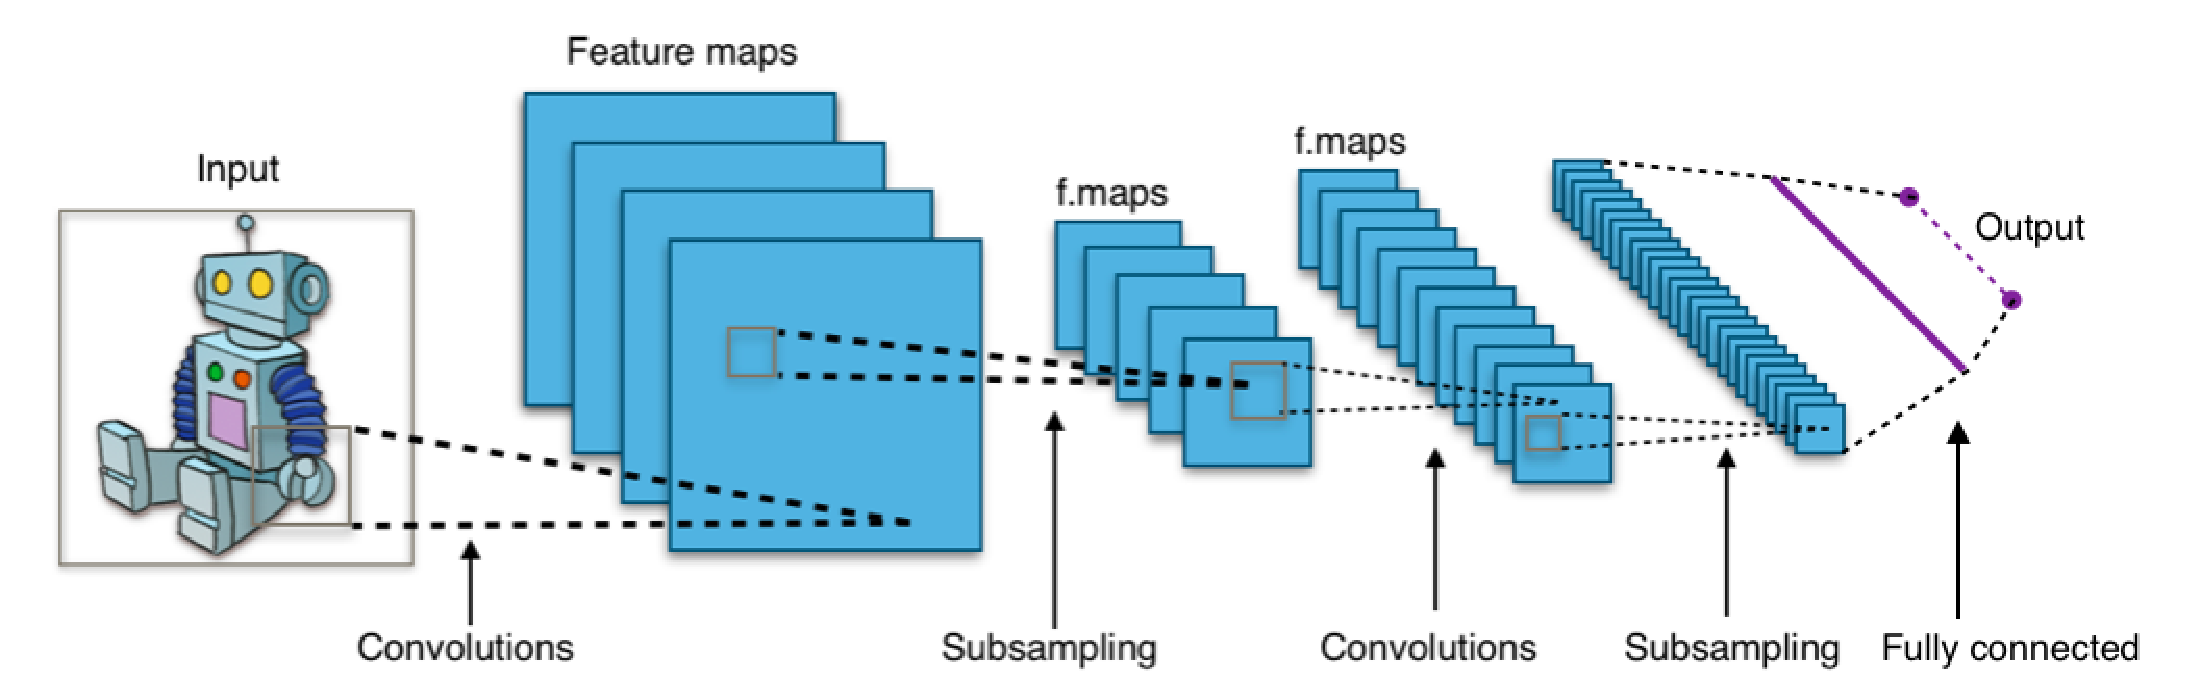
\includegraphics[width=\textwidth]{ConvolutionalNet}

  \vskip 1 cm
  \begin{center}
    \href{http://yann.lecun.com/exdb/lenet/}{\beamergotobutton{LeNet}}
  \end{center}
\end{frame}

\section{AlphaGo}

\subsection{The Policies}

\begin{frame}
  \frametitle{Supervised learning of policy networks: $p_\sigma(a|s)$}
  Predict the expert's move:
  \begin{itemize}
  \item Given board state $s$, predict probability of move $a$
  \item 13 convolutional layers
    \begin{itemize}
    \item Input: 48 features
    \item Layer 1: 192 of $5\times 5$
    \item Layers 2--12: 192 of $3\times 3$
    \item Rectifier nonlinearities
    \end{itemize}
  \item Training: 30 million positions from KGS
  \item 57\% accurate
  \item Evaluation time: 3 ms
  \end{itemize}
  \begin{tcolorbox}
    \begin{center}
      $\Delta \sigma \propto \frac{\partial \log p_\sigma(a_t|s_t)}{\partial \sigma}$
    \end{center}
  \end{tcolorbox}
\end{frame}

\begin{frame}
  \frametitle{Supervised learning of policy networks II: $p_\pi(a|s)$}
  Predict the expert's move (faster):
  \begin{itemize}
  \item Given board state $s$, predict probability of move $a$
  \item Small pattern features
  \item Training: 8 million positions from Tygem (?)
  \item 24\% accurate
  \item Evaluation time: 2 $\mu$s
  \end{itemize}
  Why? To be continued\dots
\end{frame}

\begin{frame}
  \frametitle{Reinforcement learning of policy networks: $p_\rho(a|s)$}
  Don't predict expert moves: Win!
  \begin{itemize}
  \item Start with the supervised move predictor: $\rho \leftarrow \sigma$
  \item Training: self-play vs. a previous iteration of $\rho$
  \item Result of game is $z$
  \end{itemize}
  \begin{tcolorbox}
    \begin{center}
      $\Delta \rho \propto \frac{\partial \log p_\rho(a_t|s_t)}{\partial \rho}z$
    \end{center}
  \end{tcolorbox}
  $p_\rho$ won 80\% of its games vs. $p_\sigma$
\end{frame}


\begin{frame}
  \frametitle{Reinforcement learning of value networks: $v^p(s)$}
  Predict the likelihood of winning from any board position
  \begin{itemize}
  \item $v^p(s) = \mathbb{E}\left[ z | s = s_t, a_{t\ldots T} \sim p\right]$
  \item Similar architecture to $p_\rho$, but outputs scalar $v$
  \item Trained from 30 million samples from self-play by $p_\rho(s,a)$
    \begin{itemize}
    \item Decorrelate sequences of moves
    \end{itemize}
  \end{itemize}
  \begin{tcolorbox}
    \begin{equation*}
      \Delta \theta \propto \frac{\partial v_\theta(s)}{\partial \theta}(z-v_\theta(s))
    \end{equation*}
  \end{tcolorbox}
\end{frame}


\againframe<2>{mcts}

\subsection{Move selection}


\begin{frame}
  \frametitle{Choosing a move}
  \begin{itemize}
  \item Evaluate potential new position $s'$ in 2 ways:
    \begin{itemize}
    \item $v_\theta(s')$
    \item Monte Carlo rollout (using the fast policy $p_\pi$)
      \begin{itemize}
      \item Initialise MCTS priors $\forall a$ from $p_\sigma(s',a)$ + exploration term
      \end{itemize}
    \end{itemize}
    \item Combine the evaluations ($\lambda$).
  \end{itemize}
\end{frame}



\begin{frame}
  \begin{center}
    \includegraphics[width=\textwidth]{alphago-policy-example-1}
  \end{center}
  \vskip 1 mm
  \begin{columns}
    \column{0.33\textwidth}
    Evaluation of all successors $s′$ of the root position $s$, using the value network $v_\theta(s′)$; estimated winning percentages are shown for the top evaluations.
    \column{0.33\textwidth}
    Action values $Q(s, a)$ for each edge $(s, a)$ in the tree from root position $s$; averaged over value network evaluations only ($\lambda = 0$).
    \column{0.33\textwidth}
    Action values $Q(s, a)$, averaged over rollout evaluations only ($\lambda = 1$).
  \end{columns}
\end{frame}

\begin{frame}
  \begin{center}
    \includegraphics[width=\textwidth]{alphago-policy-example-2}
  \end{center}
  \vskip 1 mm
  \begin{columns}
    \column{0.33\textwidth}
    Move probabilities directly from the SL policy network, $p_\sigma(a|s)$; reported as a percentage (if above 0.1\%)
    \column{0.33\textwidth}
    Percentage frequency with which actions were selected from the root during simulations.
    \column{0.33\textwidth}
    AlphaGo's move, and the most likely continuation of the game.
  \end{columns}
\end{frame}


\section{Results}

\begin{frame}
  \frametitle{Results}
  \includegraphics[width=\textwidth]{alphago-perf}
\end{frame}


\begin{frame}
  \frametitle{Victory!}
  \begin{itemize}
  \item Beat Fan Hui 2p 5-0
  \item Beat Lee Sedol 9p 4-1
    \begin{itemize}
    \item \href{http://ps.waltheri.net/database/game/72538/}{\beamergotobutton{One of 'em!}}
    \end{itemize}
  \item $10^3$ times fewer position evaluations than Deep Blue!
    \begin{itemize}
    \item Learns to aggressively examine only a few promising moves
    \item Learns intuition for values of intermediate positions
    \item Plays like a human?
    \end{itemize}
    \item ``AlphaGo's play makes us feel free, that no move is impossible. Now everyone is trying to play in a style that hasn't been tried before.'' --Zhou Ruiyang 9p
  \end{itemize}
\end{frame}

\begin{frame}
  \frametitle{Future work}
  \begin{itemize}
  \item Ke Jie 9p
    \begin{itemize}
    \item May 23--27
    \end{itemize}
  \end{itemize}
\end{frame}

\againframe<7>{Kasparov}

\end{document}
